\documentclass{article}
\usepackage[utf8]{inputenc}
\usepackage{mathrsfs, amsmath, mathbbol, graphicx, amssymb}
% \usepackage[backref=page]{hyperref}
    % mathrsfs = símbolos: lagrangiano
        % \mathscr{L}
    % amsmath = romper ecuaciones en nuevas líneas y centrar
        % \begin{split}
        % \end{split}
    % mathbbol = Para mostrar los conjuntos numéricos
    % graphix = Para insertar imágenes
    % amssymb = Para caracterés de operación raros, como equivalente.

\setlength{\parskip}{5px}

\title{Cálculo integral: valor presente y valor futuro}
\author{
    Jorge Antonio Gómez García \\
    Emiliano Martín Lugo López \\
    Saud Antonio Morales González}
\date{22/05/2022}

\begin{document}
\maketitle
    \section{Introducción. Definición de conceptos y preámbulo al cáluclo integral}

        En este texto, aprenderá una de las aplicaciones más importantes de la integral definida a los negocios negocios y a la economía: el valor presente y futuro. Pero, antes de entrar en materia es necesario que tenga conocimiento de ciertos conceptos básicos que le ayudarán a comprender tanto los problemas de aplicación, como la importancia del uso de las integrales en estos casos.

        \subsection{Interés compuesto}

            Cuando una empresa o una persona obtienen ingresos, pueden decidir si gastarlos en el presente, o invertirlos para obtener intereses en el futuro. +
            Para entender la manera en la que estos agentes toman decisiones con respecto a su dinero, y la manera en la que el dinero genera estos intereses, es necesario que el lector conozca el concepto de \textbf{interés compuesto}:

            \begin{quote}
                Al final de cada periodo, el interés generado durante ese periodo se agrega al capital (monto invertido), de modo que también genere interés en el periodo siguiente. La fórmula básica para el valor (o monto compuesto) de una inversión después de n periodos de interés compuesto es como sigue:
            \end{quote}
            \begin{equation}
                S=P(1+r)^{n}
            \end{equation}

            \begin{quote}
                Para una cantidad de capital ($P$), proporciona el monto de capital compuesto ($S$) a una tasa de interés periódica $r$ al final del $n$ periodos.\footnote[1]{Ernest F. Haeussler, Jr, Richard S. Paul y Richard J. Wood, Matemáticas para administración y economía, trad. Jesús Elmer Murrieta Murrieta, 11a ed. (Estado de México: Pearson, 2008), 97.}
            \end{quote}

        \subsection{Flujos de ingreso y anualidades}

            Cuando un agente económico genera un ingreso al realizar una operación económica, podemos decir que tiene un \textbf{flujo de ingreso}, que incluso podrá invertir en el futuro. Así mismo, cuando hablamos del valor futuro del flujo de ingreso, o el flujo futuro, estamos habando del flujo de ingreso inicial sumado al interés que que ha acumulado en un determinado plazo de tiempo.

            Por su parte, las \textbf{anualidades} se determinan como los flujos de ingreso llevados a cabo en determinados periodos de tiempo \textbf{regulares}, dentro de un plazo específico. Un ejemplo de anualidad es el pago de un préstamo automotriz obtenido a crédito.

        \subsection{El valor presente y el valor futuro}

            Ahora bien, conceptos como el \textbf{valor presente} y el \textbf{valor futuro} de una cantidad determinada de inversión, son valores que pueden servirle para determinar la cantidad de dinero que necesita ahorrar para solicitar un crédito de automóvil o un crédito hipotecario, o para saber la cantidad de dinero suficiente necesaria tras un plan de ahorro, como la jubilación.

            \textbf{Valor presente}: Es la manera de asignar valor a cualquier activo de manera que, su cálculo se obtenga de descontar el flujo futuro en base a una tasa de rentabilidad ofrecida por alternativas de inversión comparables denominada tasa mínima.\footnote[2]{Andrea Broseta, "Valor presente y valor futuro: definición, fórmulas y ejemplos", Rankia, 29 de julio de 2021.}

            \textbf{Valor futuro}: Este es la cantidad de dinero que una inversión puede alcanzar en una fecha futura al ganar intereses a una tasa compuesta.\footnote[3]{Broseta, "Valor presente y valor futuro: definición, fórmulas y ejemplos".} Puede darse el caso en el que \textbf{conoce el valor futuro de la inversión, y lo que busca es conocer el valor presente} del capital. Para ello, puede usar la siguiente fórmula:

            \begin{equation}
                P=S(1+r)^{-n}
            \end{equation}

            \begin{quote}
                El capital P que debe invertirse a la tasa periódica r durante n periodos de interés, de modo que el monto total sea S. Este es el \textbf{valor presente} del capital final ($S$).
            \end{quote}

        \subsection{Ejemplos de aplicación previos al cálculo integral}

            \subsubsection{Sobre el valor presente}

                Suponga que depositan \$200 a una cuenta que paga el 8\% de interés compuesto anualmente. Así, usando la ecuación (1) note que la cuenta al final del tercer año valdrá:

                \begin{equation*}
                    200(1.08)^{3} = 251.94
                \end{equation*}

                Describiendo la relación entre el capital inicial y el capital final, podemos decir que este último es el \textit{valor futuro} de los \$200 que, a su vez, son el \textit{valor presente} o capital inicial.

            \subsubsection{Sobre el valor futuro}

                Imagine que debe pagar \$2,000 en tres años, y sabe que la tasa de interés que va a pagar es de 11\% de interés compuesto mensualmente.
                
                Como sabe, La frecuencia de los pagos es mensual, por lo que la cantidad de periodos en la que tiene que dividir sus pagos es de 3 años multiplicado por los meses. Es decir, tiene 36 periodos ($n = 36$). Mientras que la tasa de interés es de 11\% anual. Sin embargo, genera interés compuesto mensualmente, por lo que, usando la ecuación (2) tenemos:

                \begin{equation*}
                \begin{split}
                    P &= 2000 \left(\frac{0.11}{12}\right)^{-3(12)} \\
                    P &\approx 2000(0.0091)^{-36} \\
                    P &\approx 1443.44
                \end{split}
                \end{equation*}

                Una forma gráfica de ver el cálculo del valor presente y del valor futuro es la siguiente:

                \begin{figure}[h]
                    \centering
                    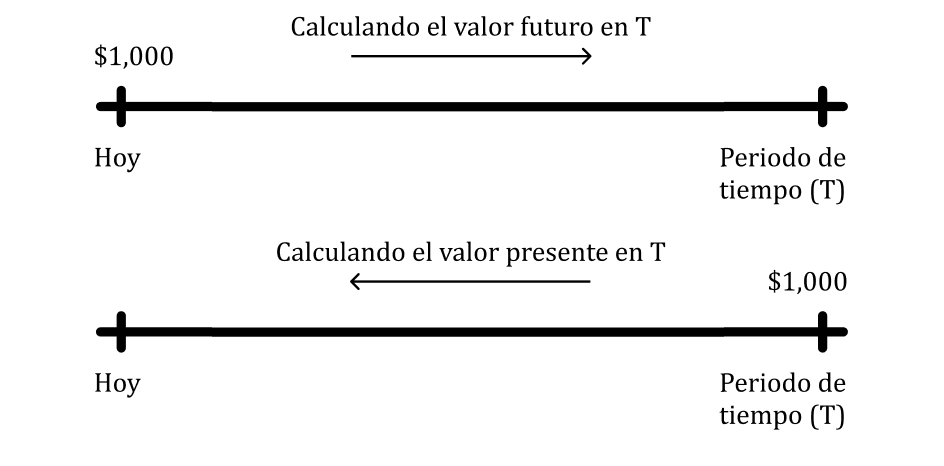
\includegraphics[width=9cm]{img_1.png}
                \end{figure}

                Esto nos lleva al planteamiento de la \textbf{ecuación de valor}. Esta es una ecuación que determina (iguala) la suma de los pagos con la suma de las deudas cuando sólo se conoce una fecha determinada.

                Imagine, por ejemplo, que se debe pagar una deuda de \$3,000 dentro de seis años, pero en lugar de eso será saldada por medio de tres pagos: \$500 ahora, \$1,500 dentro de tres años y un pago final al término de cinco años. ¿Cuál será este pago si se supone un interés de 6\% compuesto anualmente?\footnote[4]{F. Haeussler, Jr, S. Paul y J. Wood, Matemáticas para administración y economía, 203.}

                Una forma gráfica de ver este problema es la siguiente:

                \begin{figure}[h]
                    \centering
                    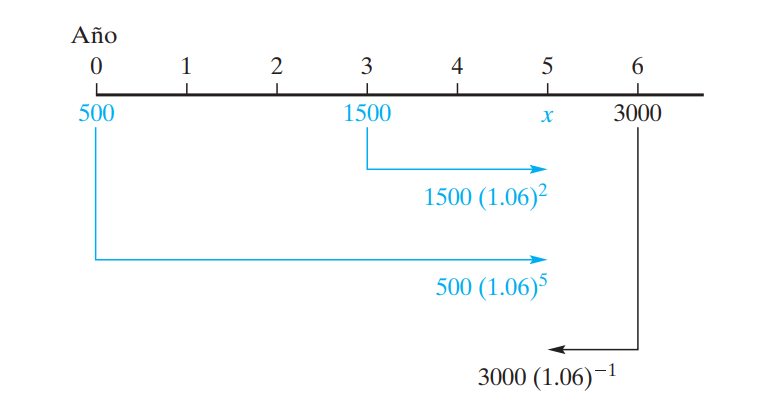
\includegraphics[width=8cm]{img_2.png}
                \end{figure}

                Por lo tanto, la función de valor planteada es la siguiente:

                \begin{equation*}
                    \begin{split}
                        500(1.06)^{5} + 1500(1.06)^{2} + x &= 3000(1.06)^{-1} \\
                        x &= 3000(1.06)^{-1} - 500(1.06)^{5} - 1500(1.06)^{2} \\
                        x &\approx 475.68
                    \end{split}
                \end{equation*}

                

                
        \section{La integral definida y el valor presente y futuro}

            Ahora bien, imagine que divide en $\Delta t$ subperiodos el periodo $t$ la duración de cada periodo tiende a cero. En este caso, decimos que el capital invertido se capitaliza continuamente.

            Cuando esto pasa, la fórmula para obtener, el valor futuro por ejemplo, viene dado por las fórmulas:

            - Para conocer el valor futuro:
            \begin{equation}
                V_F = V_P \cdot e^{it}
            \end{equation}
            
            - Para conocer el valor presente:
            \begin{equation}
                V_P = V_F \cdot e^{-it}
            \end{equation}

            \subsection{¿Por qué $e$?}

            Imagine que tiene un capital de \$100, y un banco le ofrece a usted una tasa de interés del 100\% al cabo de un año por invertir su dinero ahí. Es decir, que al finalizar el año, usted tendrá \$200 en su cuenta bancaria. Ahora, suponga que el banco le pregunta si estaría dispuesto a invertir esos mismos \$100, pero que ahora va a invertir en dos periodos de seis meses cada uno. En lugar de ofrecerle el 100\% de interés en un año, le ofrece el 50\% de interés cada 6 meses. Usted decide invertir su dinero, y se da cuenta, que al transcurrir el periodo de 1 año, en su cuenta bancaria se encontrarán \$225 pesos.

            ¿Qué significa esto?, ¿eso quiere decir que si el banco le ofrece invertir su dinero en periodos infinitesimales durante un año, usted obtendrá rendimientos inifitos? El número de Euler, o $e$, representa justo eso. Si usted invierte en periodos infinitesimales su dinero, en el periodo de un año, podrá multiplicarlo por un máximo de aproximadamente 2.7146. Esto es el número $e$, y está definido por la fórmula:

            \begin{equation}
                e=\lim _{n \rightarrow \infty}\left(1+\frac{1}{n}\right)^{n}
            \end{equation}

            Dónde, en nuestro ejemplo, $n$ llegó a 2 (dos divisiones del periodo de tiempo), pero, mientras más dividamos este intervalo (en nuestro caso, un año) más nos acercaremos al número $e$.

            \subsection{Ejemplos de aplicación con cálculo integral}

                \subsubsection{Sobre el valor presente}

                    La fórmula para calcular el \textbf{valor presente} es la siguiente:

                    \begin{equation}
                        V_P=\int_{0}^{T} f_{(t)} e^{-r t} d t
                    \end{equation}

                    \begin{quote}
                        Dónde $V_P$ es el número de dólares invertidos, $T$ la cantidad de tiempo (años, por ejemplo), $f_{(t)}$ es la tasa continua y $r$ la tasa de interés capitalizada continuamente.
                    \end{quote}

                    \textbf{- Ejemplo:}

                    Una persona debe decidir entre dos estrategias de ahorro para su retiro. El primer instrumento financiero tiene un costo de \$3,150,000 y se espera que genere un flujo de ingresos continuo a una tasa de $f_{1}(t)=1000e^{0.1t}$ pesos. El segundo instrumento tiene un costo de \$100 y se espera que genere un ingreso a una tasa de $f_{2}(t)=100e^{0.05t}$. Si la tasa de interés anual permanece fija a 11\% capitalizada continuamente durante los siguientes 45 años, ¿cuál es la inversión que generará más ingreso durante ese periodo?¿Conviene ahorrar en estos instrumentos?
                        
                    \begin{equation*}
                    \begin{split}
                        V_{P_{1}}&=\int_{0}^{45} (1000e^{0.1t})e^{-0.11t} dt \\
                        V_{P_{1}}&=1000\int_{0}^{45}e^{-0.01t} dt \\
                        V_{P_{1}}&=\frac{-1000e^{-.01}}{.01}\Biggr|_{0}^{45} \\
                        V_{P_{1}}&=\left[ \frac{-1000e^{(-.01)(.45)}}{.01}+\frac{1000e^{(-.01)(0)}}{.01}\right] \\
                        V_{P_{1}}&= \frac{-1000e^{-.45}}{.01}+\frac{1000}{.01}\\
                        V_{P_{1}}&=\$36\ 237.1848 \\\\
                    \end{split}
                    \end{equation*}

                    \begin{equation*}
                    \begin{split}
                        V_{P_{2}}&=\int_{0}^{45} (100e^{.05t})e^{-.11t} dt \\
                        V_{P_{2}}&=100\int_{0}^{45}e^{-.06t} dt \\
                        V_{P_{2}}&=\frac{-100e^{-.06}}{.06}\Biggr|_{0}^{45} \\
                        V_{P_{2}}&=\left[ \frac{-100e^{(-.06)(.45)}}{.06}+\frac{100e^{(-.06)(0)}}{.06}\right] \\
                        V_{P_{2}}&= \frac{-100e^{-2.7}}{.06}+\frac{100}{.06}\\
                        V_{P_{2}}&=\$1\ 554.6574 \\
                    \end{split}
                    \end{equation*}

                    \textbf{Respuesta}\
                    El instrumento 1 genera más ingreso total, pero debido al costo inicial que tiene, solamente conviene ahorrar en el instrumento financiero 2.

                \subsubsection{Sobre el valor futuro}

                    La fórmula para calcular el \textbf{valor futuro} es la siguiente:

                    \begin{equation}
                    \begin{split}
                        V_F &=\int_{0}^{T} f_{(t)} e^{r(T-t)} d t \\
                        V_F &= e^{r T} \int_{0}^{T} f_{(t)} e^{-r t} d t
                    \end{split}
                    \end{equation}

                    \begin{quote}
                        Dónde $V_F$ es el número de dólares esperados tras la inversión, $T$ la cantidad de tiempo (años, por ejemplo), $f_{(t)}$ es la tasa continua y $r$ la tasa de interés capitalizada continuamente.
                    \end{quote}

                    \textbf{- Ejemplo:}

                    Se transfiere dinero a una cuenta a una tasa constante de \$38,520 por año. La cuenta gana interés a una tasa anual de 8\% capitalizada continuamente.¿Cuánto habrá en la cuenta al cabo de 3 años? Suponga que la cantidad se deposita continuamente en la cuenta.
                    \begin{equation*}
                    \begin{split}
                        F &= \int_{0}^{2} 38520e^{.08(2-t)} dt \\
                        V_F &= 38520e^{.16}\int_{0}^{2}e^{-.08t} dt \\
                        V_F &= \frac{-38520e^{.16}}{.08}(e^{-.08t})\Biggr|_{1}^{9} \\
                        V_F &= \left[ \frac{-38520e^{.16}}{.08}(e^{-.16})+\frac{38520e^{.16}}{.08}(e^{0})\right] \\
                        V_F &= \frac{-38520}{.08}+\frac{38520e^{.16}}{.08}\\
                        V_F &=\$83\ 545.48
                    \end{split}
                    \end{equation*}
                    
        \section{Ejercicios de práctica}

        \begin{itemize}
            \item Alberto trata de decidir entre dos inversiones. La primera cuesta \$10 000 y se espera que genere un flujo de ingresos continuo a una tasa de $f_1(t)=2\ 500e^{0.03t}$ dólares por año. La segunda inversión es una anualidad que cuesta \$10 000 para comprar y generar ingreso a una tasa constante de $f_2(t)=4\ 000$ dólares por año. Si la tasa de interés anual permanece fija a 6\% capitalizada continuamente durante los próximos 4 años. ¿Cuál inversión generará más ingreso neto durante este periodo?
            
            \item Suponga que transfiere dinero a una cuenta, a una tasa constante de \$1 200 por año. La cuenta gana intereses a una tasa anual de 8\% capitalizada continuamente. ¿Cuanto habrá en la cuenta al cabo de 2 años? Suponga que la anualidad se deposita continuamente en la cuenta.
            
            \item Javier debe decidir entre dos estrategias de ahorro para su retiro. El primer instrumento financiero tiene un costo de \$1,150,000 y se espera que genere un flujo de ingresos continuo a una tasa de $f_{1}(t)=800e^{0.04t}$ pesos. El segundo instrumento tiene un costo de \$1 000 y se espera que genere un ingreso a una tasa de $f_{2}(t)=120e^{0.06t}$. Si la tasa de interés anual permanece fija a 8\% capitalizada continuamente durante los siguientes 30 años, ¿cuál es la inversión que generará más ingreso durante ese periodo?¿Conviene ahorrar en estos instrumentos?
            
            \item Julieta quiere decidir entre dos inversiones. La primera cuesta \$7 000 y se espera que genere un flujo de ingresos continuo a una tasa de $f_1(t)=5\ 000e^{0.04t}$ dólares por año. La segunda inversión es una anualidad que cuesta \$14 000 para comprar y generar ingreso a una tasa constante de $f_2(t)=6\ 000$ dólares por año. Si la tasa de interés anual permanece fija a 7\% capitalizada continuamente durante los próximos 6 años. ¿Cuál inversión generará más ingreso neto durante este periodo?
            
            \item Si transfiere dinero a una cuenta, a una tasa constante de \$4 000 por año.que gana intereses a una tasa anual de 4\% capitalizada continuamente. ¿Cuanto habrá en la cuenta al cabo de 5 años? Suponga que la anualidad se deposita continuamente en la cuenta.
            
        \end{itemize}

        \section{Bibliografía}
            
            Broseta, Andrea.  ``Valor presente y valor futuro: Definición, fórmulas y ejemplos''. Rankia, 29 de julio de 2021. recuperado de https://www.rankia.cl/blog/

            F. Haeussler, Jr, Ernest, Richard S. Paul y Richard J. Wood. Matemáticas para administración y economía. Traducido por Jesús Elmer Murrieta Murrieta. 11a ed. Estado de México: Pearson, 2008.

            IngeChay Clases. "Cálculo integral - Valor presente de un ingreso continuo 2020". YouTube, 26 de junio de 2020. Video, 16:40. https://www.youtube.com/watch?v=Zld8WtqWzIY.


\end{document}